\documentclass[11pt]{article}
\pagestyle{plain} 
\usepackage[text={6.5in,9.5in},centering]{geometry}
\usepackage{amsmath}
\usepackage{graphicx}
\usepackage{caption}
\usepackage{float}


%%%%%%%%%%%%%%%%%%%%%%%%%%%%%%%%%%%%%%%%%%%%%%%%%%%%%%%%%%%%%%%%%%%%%%%
% Don't touch anything above here!
%%%%%%%%%%%%%%%%%%%%%%%%%%%%%%%%%%%%%%%%%%%%%%%%%%%%%%%%%%%%%%%%%%%%%%%
\counterwithin{equation}{enumi}
\begin{document}


%%%%%%%%%%%%%%%%%%%%%%%%%%%%%%%%%%%%%%%%%%%%%%%%%%%%%%%%%%%%%%%%%%%%%%%
% Fill in your name, make sure the rest is correct
%%%%%%%%%%%%%%%%%%%%%%%%%%%%%%%%%%%%%%%%%%%%%%%%%%%%%%%%%%%%%%%%%%%%%%%
\noindent Nathan Burwig \\
Math 87 HW 1 \\
Due 2/02/22 

\hrulefill



%This is how you make a list....
\begin{enumerate}


%%%%%%%%%%%%%%%%%%%%%%%%%%%%%%%%%%%%%%%%%%%%%%%%%%%%%%%%%%%%%%%%%%%%%%%
% Problem 1
%%%%%%%%%%%%%%%%%%%%%%%%%%%%%%%%%%%%%%%%%%%%%%%%%%%%%%%%%%%%%%%%%%%%%%%
\item 
\begin{enumerate}
    \item How much of a discount will maximize the gyms profits on this special?
    Model the question as a single-variable optimization problem \\
    
    Note: for all calculations, I assume n = 100    
    
    We know we want to maximize the profits of the gym with this discount.
    Thus, we need to find out what the optimal discount would be to maximize
    profts. The first step to doing this is to find the profit function, in
    terms of the variable we wish to optimize ($k=$ \$ amount of discount,
    $n=$ number of people purchasing membership)
    
    This relationship can be modelled as follows:
    
    \begin{equation}
        \label{eqn:profit}
        P(k)=n\left( 1800 - k \right) \left(1 + \frac{0.15}{100}k \right)
    \end{equation}
    
    From here, we want to maximize profit against our variable k, so we can
    differentiate and solve to see...
    
    \begin{align*}
        \frac{dP(k)}{dk} &= n(1.7-0.003k)\\
        0 &= n(1.7-0.003k)\\
        k &= 566.667
    \end{align*}
    
    Thus our optimal discount is \$566.67 leading to a total subscription price of
    \$1,233.00 and a net profit of \$226,166.65.
    
    \item Compute the sensitivity of the optimal discount and the corresponding profit to the
    15\% assumption. \\
    
    We want to know the sensitivity of the profit relative to change in the
    percentage increase of subscriptions as a result of the discount. In order to
    find this, we will need to take our first profit formula and parameterize the
    15\% assumption as a variable. Doing so yields...
    
    $$P(k,m)=n\left(1800-k\right) \left(1 + \frac{m}{100} k\right)$$
    
    We can differentiate this formula and solve for $k(m)$:
    
    \begin{equation}
    k(m) = \frac{50 (18m - 1)}{m}
    \end{equation}
    
    Now we can find the sensitivity of the profit to the discount using the
    following formula:
    
    $$S(k,m) = \frac{dk(m)}{dm} \frac{m}{k(m)} $$
    
    Doing so yields a formula which we can solve for the 15\% assumption to find a
    sensitivity of...
    
    $$S(k,m) = \frac{1}{18m - 1} \Rightarrow S(k,m) = 0.588$$
    
    \newpage
    \item Suppose that the special only generates a 10\% increase in sales per \$100. What is the
    effect? \\
    
    We can calculate the exact effect that would be had on the profit and the
    optimal discount by utilizing equation $(1.2)$ and plugging in for $m = .10$
    then calculating the profit from the optimal discount. Doing so yields...
    
    \[k(0.10) = 400.00\]
    
    Thus the optimal discount is \$400 meaning our total profit is \$196,000.00. So
    changing our assumption from .15 to .10, decreased our profit, but in total was
    a net profit gain from the \$180000.00 that would have been earned if not for
    the discount.
    
    \item Under what circumstances would an offer of a special cause a reduction in profit (your
    answer should be quantitative)? \\
    
    If we want to know when the discount would result in a decrease in profit, we
    can just calculate where the critical point of the profit function is with
    respect to our parameter m given the optimal discount.
    
    \begin{align*}
        \frac{dP}{dm} &= \frac{d}{dm} \left[n(1800 - k)(1+ \frac{m}{100} k)\right] \\
        0 &= 25\left(324 - \frac{1}{m^2} \right)n \\
        m &= \frac{1}{18} \approx .055
    \end{align*}
    
    So when the increase in customers per \$100 discount is at approximately 5.5\%,
    having a discount would no longer be profitable. \\
    

\end{enumerate} 


%%%%%%%%%%%%%%%%%%%%%%%%%%%%%%%%%%%%%%%%%%%%%%%%%%%%%%%%%%%%%%%%%%%%%%%
% Problem 2
%%%%%%%%%%%%%%%%%%%%%%%%%%%%%%%%%%%%%%%%%%%%%%%%%%%%%%%%%%%%%%%%%%%%%%%
\item 
\begin{enumerate}
    \item Find the optimal temperature and pH level in the allowed range. \\

    Given that we already know what function we desire to optimize, we can
    immediately jump into optimization. We can optimize by differentiating with
    respect to each variable and setting each equation to zero. This will give
    us a system of equations which we can solve to find our optimal value. I
    will hold off on considering the bounds of this function, until after an
    initial optimal value has been found. A boundary analysis can be completed
    if the optimal value is not within bounds.

    We start be differentiating the following function...
    \begin{equation}
        F(H,T) = -0.038T^2 - 0.223TH - 10.982H^2 + 7.112T + 60.912H - 328.896
    \end{equation}
    
    Differentiating with respect to both variables yields...

    \begin{align*}
        \frac{\partial F}{\partial T} &= -0.076T - 0.223H + 7.112 \\            
        \frac{\partial F}{\partial H} &= -0.223T - 21.964H + 60.912             
    \end{align*}

    This system can be arranged into a matrix equation that looks like the
    following:
    \[
    \begin{bmatrix}
        0.076 & 0.223\\
        0.223 & 21.964
    \end{bmatrix}
    \begin{bmatrix}
        T \\
        H
    \end{bmatrix}
    =
    \begin{bmatrix}
        7.112 \\
        60.912
    \end{bmatrix}
    \]

    This system can be solved (chose to do so using numpy arrays) and doing to
    yeilds an optimal T and H value of $T = 88.065$, $H = 1.879$.

    Notably, these values are completely within the bounds given by the
    problem, so further analysis of optimal values is not required.

    \item Use matplotlib to produce a graph and a contour plot of the percentage of the powder
    function F (H, T ).\\

    We can use matplotlib to plot our graph and get a couple angles like
    so:

    \begin{figure}[h]
        \centering
        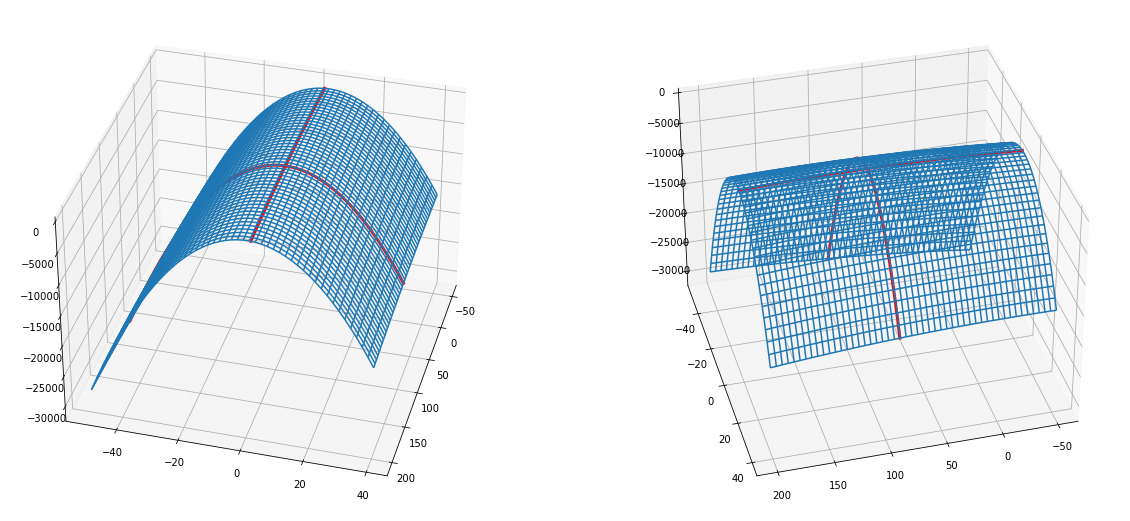
\includegraphics[scale=.34]{output1.png}
        \caption{A couple of plots of $F(H,T)$ to give an idea\\ of the shape and
                 maximum point}
    \end{figure}


    Now we can include a contour plot, which is helpful, in this case, for
    verifying our optimal value is in fact in the correct area.

    \begin{figure}[h]
        \centering
        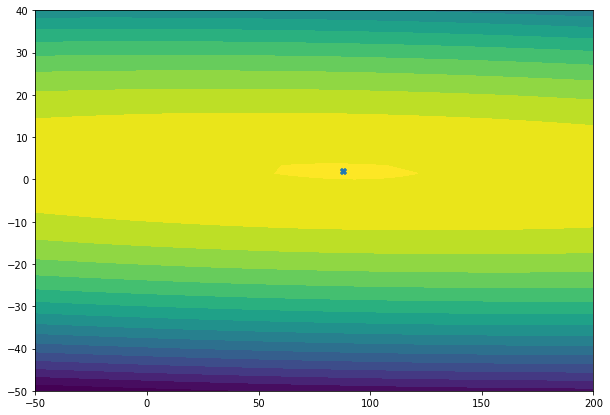
\includegraphics[scale=.34]{contour.png}
        \caption{A contour plot with the corresponding maximal\\ value marked by the 
                 blue x}
    \end{figure}
    \newpage

\end{enumerate}

%%%%%%%%%%%%%%%%%%%%%%%%%%%%%%%%%%%%%%%%%%%%%%%%%%%%%%%%%%%%%%%%%%%%%%%
% Problem 3
%%%%%%%%%%%%%%%%%%%%%%%%%%%%%%%%%%%%%%%%%%%%%%%%%%%%%%%%%%%%%%%%%%%%%%%

\item
\begin{enumerate}
    \item The Hardy-Weinberg principle states that p, q, and r are fixed from generation to
    generation, as are the frequencies of the different genotypes. Under this assumption,
    what is the probability that an individual has genotype AA? BB? OO? What is the
    probability of an individual having two different genes?i \\

    Given the Hardy-Weinberg principle, we know that the total poplution can be
    represented in as $(p + q + r)^2$, which means that the total probability
    of an individual having two different genes can be represented in any of the 
    following ways:

    \[\frac{2pq}{(p+q+r)^2} = \frac{2pr}{(p+q+r)^2}  = \frac{2qr}{(p+q+r)^2} \]

    And the probability of having either AA, BB, or OO can be given as...

    \[\frac{p^2}{(p+q+r)^2} = \frac{q^2}{(p+q+r)^2}  = \frac{r^2}{(p+q+r)^2} \]
    
    \item Find the maximum percentage of the population that can have two different genes
    under the Hardy-Weinberg principle in two different ways, by directly maximizing a
    function of only two variables and by using the method of Lagrange
    multipliers. \\

    We will first show how to solve this using the normal mehtod of
    optimization...

    We know:

    \[F(p,q,r) = 2pq + 2pr + 2qr\]

    But also that, due to the Hardy-Weinberg principle, $r = 1 - p - q$,
    thus...

    \[F(p,q) = 2pq + 2p(1-p-q) + 2q(1-p-q)\]

    We can then differentiate in terms of $p$ and $q$ to get a system of
    equations which we can then solve.
    \begin{align*}
        \frac{\partial F}{\partial q} &= -4q - 2p + 2 \\
        \frac{\partial F}{\partial p} &= -2q - 4p + 2
    \end{align*}


    Setting the above system equal to zero results in a solvable system of
    equations. The solutions to which are $p=0.333$ and $q=0.333$, which, when
    plugged back into $p + r + q = 1$ means that $r=0.333$ also.

    We can now solve by method of Lagrange multipliers. The first step will be
    to set up our expression in terms of Lagrange multipliers.
    \begin{align*}
        F(p,q,r,\lambda) &= f(p,q,r) - \lambda(c-g(p,q,r)) \\
                   &= 2(pq + pr + qr) - \lambda(1-p-q-r)
    \end{align*}

    We can then differentiate this with respect to $p, q, r$, and $\lambda$...
    \begin{align*}
        \frac{\partial F}{\partial p} &= 2q + 2r + \lambda,\;\;\;  
        \frac{\partial F}{\partial q} = 2p + 2r + \lambda \\ 
        \frac{\partial F}{\partial r} &= 2p + 2q + \lambda, \;\;\;
        \frac{\partial F}{\partial \lambda} = p + q + r - 1
    \end{align*}

    From here, we set all of these equations to 0 and solve the system as a
    matrix equation (again, done through numpy). The result is the following
    vector $\hat{p}$.
    \[
    \begin{bmatrix}
        0.333 \\
        0.333 \\
        0.333 \\
        -1.333
    \end{bmatrix}
    \]

    Which, from top to bottom, are the values of $p, q, r,$ and $\lambda$.
    
    We can see immediately, that this result is in agreement with our previous
    result using an alternative method.

    \item Can you say what the Lagrange multiplier represents in the above
        example?\\

    To be completely honest, I'm not entirely sure I understand what the
    Lagrange multiplier represents exactly in this context. I know that the
    lagrange multiplier, is equal to the "shadow price" which means that
    formally $\lambda$ in this case is rate of change of the probability
    relative to our constraing (the Hardy-Weinberg Principle).

    What that means in this context, though, I'm not exactly sure. I suppose it
    could indicate the expected change in the optimal percentages if there were
    a fourth blood type, but given the infinitesimal nature of the value of
    $\frac{\partial F}{\partial c}$ I don't entirely understand how that would
    work.
    


\end{enumerate}







\end{enumerate}
\end{document} 
